\documentclass[11pt,oneside]{article}
\usepackage[utf8]{inputenc}
\usepackage[a4paper,top=2cm,left=2cm,right=2cm,bottom=2cm]{geometry}
\usepackage{import}
\usepackage[T1]{fontenc}
\usepackage[german,ngerman]{babel}
\usepackage[table]{xcolor}
\usepackage{amsthm, esvect}
\usepackage{mathtools}
\RequirePackage{amssymb, amsfonts, amsmath, latexsym, verbatim, xspace}
\usepackage{systeme}
\usepackage{multicol}
\usepackage{multirow}
\usepackage{framed}
\usepackage{array}
\usepackage{ragged2e}
\usepackage{graphicx}
\usepackage{pdflscape}
\usepackage{epstopdf}
\usepackage{booktabs}
\usepackage{pdfpages}
\usepackage{float} % Allows putting an [H] in \begin{figure} to specify the exact location of the figure
\usepackage{wrapfig} % Allows in-line images such as the example fish picture
\usepackage{tikz, graphicx} % tikz
\usepackage[position=top]{subfig}
\usepackage[bookmarks=true]{hyperref}%Links
\usepackage{enumerate}
\usepackage{enumitem}
\usepackage[german,ruled,vlined,linesnumbered,algosection]{algorithm2e}
\usepackage[labelfont=sf]{caption}
\usepackage{lmodern}
\usepackage{lscape}
\usepackage{tabularx}
\usepackage{systeme}
\usepackage{hhline}
\usepackage{subfiles}
\usepackage{stackengine}
\usepackage{setspace}
\usepackage{MnSymbol}
\usepackage{tcolorbox}
\usepackage{bbm}
\usepackage{url}
\usepackage{xparse}
\usepackage{sectsty}
\usepackage{array}
\usepackage{ragged2e}
\usepackage{listings} %Stellt Code-Snippets sauber dar

% definiert die Sprache
\selectlanguage{German}

% add command for different dates in Swiss fashion
\newcommand{\monthwordlong}[1]{\ifcase#1 \or Januar\or Februar\or März\or April\or Mai\or Juni\or Juli\or August\or September\or Oktober\or November\or Dezember\fi}
\newcommand{\monthwordshort}[1]{\ifcase#1\or Jan\or Feb\or Mar\or Apr\or Mai\or Jun\or Jul\or Aug\or Sept\or Okt\or Nov\or Dez\fi}
\newcommand{\datelong}{\number\day.\:\monthwordlong{\the\month}\:\number\year}
\newcommand{\dateshort}{\number\day.\:\monthwordshort{\the\month}\:\number\year}

% define color of links inside a text
\definecolor{linkblue}{RGB}{0, 0, 80}
\definecolor{plotblue}{RGB}{100, 100, 255}
\definecolor{myblue}{RGB}{8,164,214}
\definecolor{myred}{RGB}{143,42,41}
\definecolor{forestgreen}{RGB}{34,139,34}
\definecolor{highdive}{RGB}{10,169,194}
\definecolor{charcoal}{RGB}{74,74,74}
\hypersetup{
	colorlinks=true,
	linkcolor=linkblue,
	filecolor=magenta,
	urlcolor=plotblue,
	citecolor=linkblue,
	pdfpagemode=FullScreen,
}


\lstdefinestyle{mystyle}{ % definiert den style des Code-Snippets
	%backgroundcolor=\color{backcolour},
	%commentstyle=\color{codegreen},
	%keywordstyle=\color{magenta},
	%numberstyle=\tiny\color{codegray},
	%stringstyle=\color{codepurple},
	basicstyle=\ttfamily\footnotesize,
	breakatwhitespace=false,
	breaklines=true,
	captionpos=b,
	keepspaces=true,
	%numbers=left,
	%numbersep=5pt,
	showspaces=false,
	showstringspaces=false,
	showtabs=false,
	tabsize=4
}
\lstset{style=mystyle}
\usepackage{fancyhdr}

\tcbuselibrary{breakable,skins}
\usetikzlibrary{mindmap,trees}
\newlength\tindent
\setlength{\tindent}{\parindent}
\setlength{\parindent}{0pt}
\renewcommand{\indent}{\hspace*{\tindent}}

\makeatletter
\def\ifEmpty#1{\def\@temp{#1}\ifx\@temp\@empty}
\makeatother

\sectionfont{\underline}
\usetikzlibrary{arrows, petri, topaths, graphs}


% =================== BEISPIEL ====================
\theoremstyle{definition}
\newtheorem{beispiel}{Beispiel}
\renewcommand{\thebeispiel}{\arabic{beispiel}}

% =================== AUFGABE =====================
\newcounter{aufg}[section] % Zähler für die Umgebungen

\newenvironment{aufgabe}[1][]{%
    \refstepcounter{aufg}% Inkrementiere den Zähler
    \begin{tcolorbox}[%
        enhanced,
        overlay unbroken and first={\mytitleaufg[#1]}, % Titelleiste mit Icons wird nicht über Seite gebrochen
        colframe=black,
        boxrule=0pt,
        breakable,
        top=15pt,
        before=\vskip18pt,
    ]
}{%
    \end{tcolorbox}
}

\newcommand{\mytitleaufg}[1][]{% Definiert die Titelleiste und Icons
    \node[fill=black!20,
        rounded corners,
        draw=black,
        text=black,
        line width=1pt,
        inner sep=4pt,
        anchor=west,
        xshift=12pt]
        at (frame.north west){\bfseries Aufgabe \thesection.\theaufg.\ifEmpty{#1}\else\emph{ (#1)}\fi}; % Titel, letzter Teil mit ifempty testet ob #1 leer und macht Klammern und Titel, falls Titelargument übergeben wird bzw. falls #1 leer erscheint nichts - auch keine Klammern

    \node[% Icon
        rounded corners,
        text=black,
        fill=black,
        line width=0pt,
        inner sep=3pt,
        anchor=west,
        xshift=5pt,
        % yshift=-35pt
        ]
        at (frame.north east){
\includegraphics[width=24pt]{../../../Header/Icons/aufgabeicon.png}};
}

% =================== DEFINITION ==================
\newcounter{def}[section] % Zähler für die Umgebungen

\newenvironment{definition}[1][]{%
    \refstepcounter{def}% Inkrementiere den Zähler
    \begin{tcolorbox}[%
        enhanced,
        drop shadow southeast,
        overlay unbroken and first={\mytitledef[#1]}, % Titelleiste mit Icons wird nicht über Seite gebrochen
        colback=blue!5!white,
        colframe=blue!75!black,
        boxrule=2pt,
        breakable,
        top=15pt,
        before=\vskip18pt,
    ]
}{%
    \end{tcolorbox}
}

\newcommand{\mytitledef}[1][]{% Definiert die Titelleiste und Icons
    \node[fill=blue!40!white,
        rounded corners,
        draw=black,
        text=black,
        line width=1pt,
        inner sep=4pt,
        anchor=west,
        xshift=12pt]
        at (frame.north west){\bfseries Definition \thesection.\thedef.\ifEmpty{#1}\else\emph{ (#1)}\fi}; % Titel, letzter Teil mit ifempty testet ob #1 leer und macht Klammern und Titel, falls Titelargument übergeben wird bzw. falls #1 leer erscheint nichts - auch keine Klammern

    \node[% Icon
        rounded corners,
        text=black,
        fill=black,
        line width=0pt,
        inner sep=3pt,
        anchor=west,
        xshift=5pt,
        % yshift=-35pt
        ]
        at (frame.north east){
\includegraphics[width=24pt]{../../../Header/Icons/definitionicon.png}};
}

% =================== NOTATION ====================
\newcounter{nota}[section] % Zähler für die Umgebungen

\newenvironment{notation}[1][]{%
    \refstepcounter{nota}% Inkrementiere den Zähler
    \begin{tcolorbox}[%
        enhanced,
        drop shadow southeast,
        colback=yellow!5!white,
        colframe=yellow!75!black,
        overlay unbroken and first={\mytitlenota[#1]},   % Titelleiste mit Icons wird nicht über Seite gebrochen
        boxrule=2pt,
        breakable,
        top=15pt,
        before=\vskip18pt,
    ]
}{%
    \end{tcolorbox}
}

\newcommand{\mytitlenota}[1][]{% Definiert die Titelleiste und Icons
    \node[fill=yellow!40!white,,
        rounded corners,
        draw=black,
        text=black,
        line width=1pt,
        inner sep=4pt,
        anchor=west,
        xshift=12pt]
        at (frame.north west){\bfseries Notation \thesection.\thenota.\ifEmpty{#1}\else\emph{ (#1)}\fi}; % Titel, letzter Teil mit ifempty testet ob #1 leer und macht Klammern und Titel, falls Titelargument übergeben wird bzw. falls #1 leer erscheint nichts - auch keine Klammern

    \node[% Icon
        rounded corners,
        text=black,
        fill=black,
        line width=0pt,
        inner sep=3pt,
        anchor=west,
        xshift=5pt,
        % yshift=-35pt
        ]
        at (frame.north east){
\includegraphics[width=24pt]{../../../Header/Icons/definitionicon.png}};
}

% =================== SATZ ========================
\newcounter{satz}[section]  % creates a counter and resets it after each chapter

\newenvironment{satz}[1][]{   % Hauptbox mit Satz drin
    \refstepcounter{satz}
    \begin{tcolorbox}[%
        enhanced,
        colback=red!5!white,
        fuzzy halo=2mm with gray,
        colframe=red!75!black,
        overlay unbroken and first={\mytitlesatz[#1]},   % Titelleiste mit Icons wird nicht über Seite gebrochen
        boxrule=2pt,
        breakable,
        top=15pt,
        before=\vskip18pt,
    ]
}{%
    \end{tcolorbox}
}

\newcommand{\mytitlesatz}[1][]{                     % Macht Titelbox und Icons
   \node[fill=red!90!white,
      rounded corners,
      draw=black,,
      text=black,
      line width=1pt,
      inner sep=4pt,
      anchor=west,
      xshift=12pt]
   at (frame.north west){\bfseries Satz \thesection.\thesatz.\ifEmpty{#1}\else\emph{ (#1)}\fi};  % Titel, letzter Teil mit ifx testet ob #1 leer und macht Klammern und Titel, falls Titelargument übergeben wird bzw.  falls #1 leer erscheint nichts - auch keine Klammern

 \node[ % Icon
      rounded corners,
      text=black,
      fill=black,
      line width=0pt,
      inner sep=3pt,
      anchor=west,
      xshift=5pt,
%     yshift=-35pt
]
   at (frame.north east){ 
\includegraphics[width=24pt]{../../../Header/Icons/satzicon.png} };
}

% =================== BEWEIS ======================
\newenvironment{beweis}[1][]{
    \begin{tcolorbox}[
        enhanced,
        overlay unbroken and first={\mybeweis[#1]},     % Titelleiste mit Icons wird nicht über Seite gebrochen
        colback=white,
        colframe=black,
        boxrule=0pt,
        breakable,
        top=15pt,
        before=\vskip18pt,
    ]
}{
        \end{tcolorbox}
}

\newcommand{\mybeweis}[1][]{                     % Macht Titelbox und Icons
   \node[fill=white,
      rounded corners,
      draw=black,
      text=black,
      line width=1pt,
      inner sep=4pt,
      anchor=west,
      xshift=12pt]
   at (frame.north west){\bfseries Beweis \ifEmpty{#1}\else\emph{ (#1)}\fi};  % Titel, letzter Teil mit ifx testet ob #1 leer und macht Klammern und Titel, falls Titelargument übergeben wird bzw.  falls #1 leer erscheint nichts - auch keine Klammern
}

% =================== ALGORITHM ===================
\newcounter{algo}[section]  % creates a counter and resets it after each chapter

\newenvironment{algo}[1][]{   % Hauptbox mit Satz drin
    \refstepcounter{algo}
    \begin{tcolorbox}[%
        enhanced,
        drop shadow southeast,
        colback=yellow!5!white,
        colframe=yellow!75!black,
        overlay unbroken and first={\algotitle[#1]},   % Titelleiste mit Icons wird nicht über Seite gebrochen
        boxrule=2pt,
        breakable,
        top=15pt,
        before=\vskip18pt,
    ]
}{%
    \end{tcolorbox}
}

\newcommand{\algotitle}[1][]{                     % Macht Titelbox und Icons
   \node[fill=yellow!40!white,
      rounded corners,
      draw=black,
      text=black,
      line width=1pt,
      inner sep=4pt,
      anchor=west,
      xshift=12pt]
   at (frame.north west){\bfseries \ifEmpty{#1}{Ablauf}\else{#1}\fi};  % Titel, letzter Teil mit ifx testet ob #1 leer und macht Klammern und Titel, falls Titelargument übergeben wird bzw.  falls #1 leer erscheint nichts - auch keine Klammern

 \node[ % Icon
      rounded corners,
      text=black,
      fill=black,
      line width=0pt,
      inner sep=3pt,
      anchor=west,
      xshift=5pt
      % yshift=-35pt
      ]
   at (frame.north east){ 
\includegraphics[width=24pt]{../../../Header/Icons/algoicon.png} };
}

% ================ Nummerierte Multicol ================
\newenvironment{enumcols}[1][]{
    \begin{enumerate}[label=\alph*)]\begin{multicols}{#1}
}{
    \end{multicols}\end{enumerate}
}



% =================================================
\usetikzlibrary{shapes,arrows}
\tikzstyle{decision} = [diamond, draw, fill=blue!20,
    text width=6em, text badly centered, node distance=4cm, inner sep=0pt]
\tikzstyle{block} = [rectangle, draw, fill=blue!20,
    text width=8em, text centered, rounded corners, minimum height=4em]
\tikzstyle{line} = [draw, -latex']
\tikzstyle{cloud} = [draw, ellipse,fill=red!20, node distance=2cm,
    minimum height=2em]

% Karriertes Papier für Antwort
\newcommand{\karos}[1]{\begin{tikzpicture}\draw[step=0.5cm,color=gray] (0,0) grid (\linewidth,#1 cm);\end{tikzpicture}}
%%
% Header and Footer
%%
\linespread{1.2} % Line spacing
\fancypagestyle{plain}{
	\pagestyle{fancy}
	\lhead{}
	\chead{}
	\rhead{}
	\lfoot{\Autor}
	\cfoot{\Skriptname}
	\rfoot{\thepage}
	\renewcommand{\headrulewidth}{0pt}
	\renewcommand{\footrulewidth}{0.4pt}
}

\pagestyle{fancy}
\fancyhf{}
\rhead{\rightmark}
\lfoot{\leftmark}
\rfoot{\thepage}
\renewcommand{\headrulewidth}{0.2pt}
%\setlength\parindent{0pt} % Uncomment to remove all indentation from paragraphs



%%
% Math Arrows
%%
\newcommand{\same}{\ensuremath{\Longleftrightarrow}}
\renewcommand{\to}{\ensuremath{\longrightarrow}}
\newcommand{\qsame}{\quad\same\quad}
\newcommand{\dsame}{\ensuremath{:\Leftrightarrow}}
\newcommand{\qdsame}{\quad\dsame\quad}
\newcommand{\ldsame}{\ensuremath{:\Longleftrightarrow}}
\newcommand{\samedef}{\ensuremath{\us {\text{def}} \Leftrightarrow}}
\newcommand{\qsamedef}{\quad\samedef\quad}
\newcommand{\lsamedef}{\ensuremath{\us {\text{def}} \Longleftrightarrow}}
\newcommand{\qlsamedef}{\quad\lsamedef\quad}


%%
% Mengendefinitionen
%%
\newcommand{\M}{\ensuremath{\mathcal{M}}}
\newcommand{\N}{\ensuremath{\mathbb{N}}}
\newcommand{\Z}{\ensuremath{\mathbb{Z}}}
\newcommand{\Q}{\ensuremath{\mathbb{Q}}}
\newcommand{\I}{\ensuremath{\mathbb{I}}}
\newcommand{\R}{\ensuremath{\mathbb{R}}}
\newcommand{\C}{\ensuremath{\mathbb{C}}}
\renewcommand{\S}{\ensuremath{\mathbb{S}}}
\newcommand{\Prim}{\ensuremath{\mathbb{P}}}
\newcommand{\0}{\ensuremath{\emptyset}}
\renewcommand{\Re}{\ensuremath{\operatorname{Re}}}
\renewcommand{\Im}{\ensuremath{\operatorname{Im}}}
\newcommand{\strich}{\ensuremath{\big\vert}}

%%
% Mengenoperation
%%
\renewcommand{\nin}{\not\in}


%%
% Logisches Und und Oder
%%
\newcommand{\sand}{\ensuremath{\; \land \;}}
\newcommand{\sor}{\ensuremath{\; \lor \;}}
\renewcommand{\*}{\ensuremath{\cdot}}
\newcommand{\oder}{\vee}
\newcommand{\n}{\neg}
\newcommand{\und}{\wedge}


%%
% Bei Integral, Summe,... die Grenzen über bzw.
% unter das Zeichen
%%
\renewcommand{\d}[1]{\ensuremath{\operatorname{d}\!{#1}}}
\newcommand{\Sum}{\sum\limits}
\newcommand{\Prod}{\prod\limits}
\newcommand{\Min}{\min\limits}
\newcommand{\Max}{\max\limits}
\newcommand{\Lim}{\lim\limits}
\newcommand{\Inf}{\inf\limits}
\newcommand{\Sup}{\sup\limits}
\newcommand{\Liminf}{\liminf\limits}
\newcommand{\Limsup}{\limsup\limits}
%\renewcommand{\Cup}{\bigcup\limits}
%\renewcommand{\Cap}{\bigcap\limits}
\newcommand{\Otimes}{\bigotimes\limits}
\newcommand{\Oplus}{\bigoplus\limits}


%%
% Arcus Cotangens, Logarithmus
%%
\let\oldsin\sin
\renewcommand{\sin}[1]{\oldsin{\left(#1\right)}}
\let\oldcos\cos
\renewcommand{\cos}[1]{\oldcos{\left(#1\right)}}
\let\oldtan\tan
\renewcommand{\tan}[1]{\oldtan{\left(#1\right)}}
\let\oldarcsin\arcsin
\renewcommand{\arcsin}[1]{\oldarcsin{\left(#1\right)}}
\let\oldarccos\arccos
\renewcommand{\arccos}[1]{\oldarccos{\left(#1\right)}}
\let\oldarctan\arctan
\renewcommand{\arctan}[1]{\oldarctan{\left(#1\right)}}
\let\oldln\ln
\renewcommand{\ln}[1]{\oldln{\left(#1\right)}}
\newcommand{\Log}[2]{\ensuremath{\operatorname{log}_{#1}\left(#2\right)}}
\newcommand{\e}{\operatorname{e}}
\renewcommand{\exp}[1]{\ensuremath{\operatorname{\e}^{#1}}}


%%
% Griechische Buchstaben
%%
\renewcommand{\epsilon}{\ensuremath{\varepsilon}}
\renewcommand{\phi}{\varphi}
\renewcommand{\l}{\lambda}
\renewcommand{\t}{\tau}


%%
% Bezeichnungen
%%
\newcommand{\Rgn}{\R_{>0}} % R grösser Null
\newcommand{\Rad}{\operatorname{Rad}}   % Radikal
\newcommand{\kgV}{\operatorname{kgV}}   % Kleinster gemeinsame Vielfache
\newcommand{\ggT}{\operatorname{ggT}}   % Grösster gemeinsame Teiler
\newcommand{\winkel}{\sphericalangle}          % Winkelsymbol
\DeclarePairedDelimiter\abs{\lvert}{\rvert} % besserer Betrag
\makeatletter
\let\oldabs\abs
\def\abs{\@ifstar{\oldabs}{\oldabs*}}
\makeatother


%%
% Vektorgeometrie
%%
\renewcommand{\v}[1]{\vv{#1}}       % besserer Pfeil über Buchstaben
\renewcommand{\vec}[2]{\begingroup\renewcommand{\arraystretch}{1}\left(\begin{array}{c} #1 \\ #2 \end{array}\right)\endgroup}   % two dimensional vector
\renewcommand{\Vec}[3]{\begingroup\renewcommand{\arraystretch}{1}\left(\begin{array}{c} #1 \\ #2 \\ #3 \end{array}\right)\endgroup}      % three dimensional vector


%%
% Text
%%
\newcommand*{\Ueq}[1]{\mathrel{\mathop{=}\limits_{\text{#1}}}}
\newcommand*{\Oeq}[1]{\mathrel{\stackrel{\text{#1}}{=}}}
\newcommand{\utext}[2]{\underbrace{#1}_{\substack{#2}}}
\newcommand{\otext}[2]{$\overbrace{\textrm{#1}}^{\textrm{#2}}$}
\newcommand{\lineortext}[1]{\hspace{0,1cm}\underline{\hspace{0.1cm}\hphantom{#1}\hspace{0.1cm}}\hspace{0,1cm}} % Lückentext erstellen
\newcommand{\gap}[1]{\rule{#1 cm}{1pt}}


\newcommand{\Skriptname}{Folgen und Reihen}
\newcommand{\Autor}{Jonas Guler (Gu)}
\newcommand{\version}{\textit{v}1.0}

\begin{document}
\begin{titlepage}
	\clearpage
	\title{\Huge\textbf{\Skriptname} \\[1cm]}
	\author{Autor:\\ \Autor}
	\date{\normalsize {Version \version}\\ \datelong}
	\maketitle
	\thispagestyle{empty}
	\vfill
	\tableofcontents
\end{titlepage}
\pagenumbering{arabic}
%############################################################################################
\section{Einführung}
	\begin{aufgabe}
		In IQ-Test wird häufig eine Abfolge aus Zahlen präsentiert, mit der Aufgabe ein bestimmtes Muster oder die Formel zu erkennen, mit der die Abfolge gebildet wurde. Hier sind einige Beispiele solcher Abfolgen von Zahlen. Versuche, die Muster/Formel zu erraten.
		\begin{enumcols}[2]
			\item $3,9,5,15,11,33,\ldots$
			\item $1,2,4,7,11,16,\ldots$
			\item $15,9,27,20,60,52,\ldots$
			\item $2,6,18,54,162,486,\ldots$
		\end{enumcols}
		\karos{4}
		Sind solche Abfolgen von Zahlen, bzw. ihre Fortsetzung eindeutig? Findest du für eine der obigen Abfolgen eine zweite mögliche Formel?\vspace{5pt}\newline\karos{2}
	\end{aufgabe}
	Zahlenfolgen sind oftmals darum wichtig, weil mit ihnen Prognosen über die zukünftige Entwicklung eines untersuchten Prozesses gemacht werden kann. Hier eine Beispielaufgabe dazu.
	\begin{aufgabe}
		neue Einsteigsaufgabe...
	\end{aufgabe}

	Ihr kennt das Wort \glqq Folge\grqq\:vermutlich ausschliesslich als Bestandteil einer Serie auf Netflix. In diesem Abschnitt lernen wir ihm aber als mathematischen Fachbegriff kennen. Dazu werden wir ihn zuerst eindeutig definieren und danach die Bedeutungen und Auswirkungen dieses Konzepts genauer untersuchen.\newline
	Wie wir in der ersten Aufgabe gesehen haben, ist eine Folge - salopp gesagt - eine Anordnung von Zahlen, in der es nach einer bestimmten Regel oder Formel eine eindeutige Reihenfolge gibt. Im folgenden Abschnitt werden wir die genaue mathematische Definition kennenlernen.
	\newpage


\section{Folgen}
	Wir betrachten die folgenden Funktionen:\newline
	\begin{minipage}{0.47\linewidth}
		\[a:y=-x,\qquad x\in\left\{1,2,3,\ldots\right\}\]
		\begin{table}[H]
			\centering
			\begin{tabular}{c|p{6mm}|p{6mm}|p{6mm}|p{6mm}|p{6mm}|p{6mm}}
				$x$ & $1$ & $2$ & $3$ & $4$ & $5$ & $6$ \\\hline
				$f(x)$ & & & & & &
			\end{tabular}
		\end{table}
		\[b:y=\frac{6}{x+1},\qquad x\in\left\{1,2,3,\ldots\right\}\]
		\begin{table}[H]
			\centering
			\begin{tabular}{c|p{6mm}|p{6mm}|p{6mm}|p{6mm}|p{6mm}|p{6mm}}
				$x$ & $1$ & $2$ & $3$ & $4$ & $5$ & $6$ \\\hline
				$g(x)$ & & & & & &
			\end{tabular}
		\end{table}
	\end{minipage}
	\hfill
	\begin{minipage}{0.47\linewidth}
		\centering
		\begin{tikzpicture}[cross/.style={draw, cross out, minimum size=2*(#1-1pt), inner sep=0pt, outer sep=0pt}, x=1cm, y=1cm,
			>=latex,   %Voreinstellung für Pfeilspitzen
			font= \footnotesize, scale=0.8]
			%Raster zeichnen
			\draw [color=gray!50]  [step=10mm] (-0.3,-1.3) grid (6.3,4.3);
			% Achsen zeichnen
			\draw[->,thick] (-0.3,0) -- (6.8,0) node[right, below] {\normalsize $x$};
			\draw[->,thick] (0,-1.3) -- (0,4.8) node[above, left] {\normalsize $y$};
			% Achsen beschriften
			\foreach \x in {1,2,3,...,6} \draw (\x,-.1) -- (\x,.1) node[below=4pt] {$\x$};
			\foreach \y in {-1,1,2,3,...,4} \draw (-.1,\y) -- (.1,\y) node[left=4pt] {$\y$};
			% Besserer Ursprung
			\draw[color=black] (0pt,-14pt) node[right] {$0$};
			%Funktionen zeichnen:
			%\clip(-3.3,-5.3) rectangle (3.3,7.3); %Bildbereich
			%\draw[blue, smooth, domain=-9:9] plot (\x, {-1*pow(\x-3,2)+1}) node[yshift=13cm] {$$};
			%\draw[green, smooth, domain=-9:9] plot (\x, {2*pow(\x-3,2)-3}) node[] {$$};
			%\draw[red, smooth, domain=-9:9] plot (\x, {-0.4*pow(\x+3,2)+1}) node[right] {$$};
			%Beschriftung
			%\node[blue]  at (1,-5) {$p_2$};
		\end{tikzpicture}
	\end{minipage}
	\begin{definition}[reelle Zahlenfolge]
		Eine \textbf{reelle Zahlenfolge} ist eine spezielle Funktion $a:\N\to\R:\:n\mapsto a_n$, durch die jeder natürlichen Zahl $n$ eine reelle Zahl $a_n$ zugeordnet wird. Man nennt $a_n$ das $n-$te Glied der Folge und der Index $n$ die Nummer des Glieds in der Folge bezeichnet.\newline
		Die gesamte Zahlenfolge bezeichnen wir mit $a_1,a_2,a_3,\ldots$ oder $\left(a_n\right)_{n\in\N}$
	\end{definition}
	Eine reelle Zahlenfolge kann endlich viele Glieder haben, aber in den meisten Fällen besteht sie aus unendlich viele Glieder. Wir werden in den nächsten Abschnitten diese unendlichen Zahlenfolgen untersuchen. Es ist sehr mühsam eine Folge immer als Auflistung der ersten paar Elementen anzugeben. Deshalb haben sich zwei verschiedene Beschreibungsmöglichkeiten durchgesetzt. Die eine wird als \textit{explizite} Beschreibung und die andere als \textit{rekursive} Beschreibung bezeichnet.
	\begin{notation}[explizite Folge]
		Ist das allgemeine Glied $a_n$ durch einen Term in der Variablen $n$ gegeben, so heisst die Folge \textbf{explizit} beschrieben.
	\end{notation}
	\begin{beispiel}
		\[n\mapsto a_n=n^3-7n+12\]
		Berechne die ersten $5$ Glieder.
		\begin{enumcols}[5]
			\item $a_1=$ \item $a_2=$ \item $a_3=$ \item $a_4=$ \item $a_5=$
		\end{enumcols}
		Finde eine explizite Formel für die Beschreibung der Folge: $a_1=1, a_2=0, a_3=1, a_4=4, a_5=9$.\vspace{5pt}\newline\karos{1.5}
	\end{beispiel}\newpage
	Im Unterschied dazu die rekursive Beschreibung.
	\begin{notation}[rekursive Folge]
		Beschreibt man das allgemeine Glied $a_n$ einer Folge durch einen oder mehrere Vorgänger, so heisst die Folge \textbf{rekursiv} beschrieben.
	\end{notation}
	\begin{beispiel}
		\[a_1=1,\:a_{n+1}=a_n+n^2\]
		Für die ersten $5$ Glieder dieser Folge erhält man
		\begin{enumcols}[5]
			\item $a_1=$ \item $a_2=$ \item $a_3=$ \item $a_4=$ \item $a_5=$
		\end{enumcols}
		Finde eine rekursive Beschreibung der Folge: $a_1=3,a_2=5, a_3=8, a_4=12, a_5=17$.\vspace{5pt}\newline\karos{1.5}
	\end{beispiel}
	\begin{aufgabe} %DMK Ana S2 A3bcfgh,4acd,5,6,8,10,11ad
		\begin{enumerate}
			\item Suche die \textbf{explizite} Darstellung $a_n$ der gegebenen Folgen für $n\in\N$.
			\begin{enumcols}[4]
				\item $1,3,5,7,9,\ldots$
				\item $1,2,4,8,16,\ldots$
				\item $8,15,22,29,\ldots$
				\item $-13,-3,7,17,\ldots$
				\item $3,9,27,81,\ldots$
				\item $1,\frac{1}{2},\frac{1}{3},\frac{1}{4},\ldots$
				\item $\frac{-2}{3},\frac{4}{5},\frac{-8}{7},\frac{16}{9},\ldots$
				\item $\frac{4}{7},\frac{12}{15},\frac{20}{23},\frac{28}{31},\ldots$
			\end{enumcols}
			\item Berechne die beiden Glieder $a_{50}$ und $a_{51}$ der durch die ersten Glieder gegebenen Folgen, in dem du die explizite Beschreibung verwendest.
			\begin{enumcols}[2]
				\item $\frac{1}{4},\frac{3}{8},\frac{5}{12},\frac{7}{16},\frac{9}{20},\ldots$
				\item $\frac{3}{4},\frac{4}{7},\frac{1}{2},\frac{6}{13},\frac{7}{16},\frac{8}{19},\ldots$
			\end{enumcols}
			\item Beschreibe die durch die ersten Glieder gegebene Folge \textbf{rekursiv}.
			\begin{enumcols}[4]
				\item $3,7,11,15,\ldots$
				\item $6,12,24,48,\ldots$
				\item $6,13,27,55,\ldots$
				\item $4,11,32,95,\ldots$
			\end{enumcols}
			\item Von der Folge $a_n$ sind die beiden Startglieder $a_1$ und $a_2$ sowie die Rekursionsformel gegeben $a_{n+2}=2a_{n+1}-a_n$. Berechne aus den gegebenen Startgliedern die nächsten fünf Glieder, also $a_3$ bis $a_7$, und suche die explizite Darstellung für das allgemeine Glied $a_n$.
			\begin{enumcols}[4]
				\item $a_1=3,a_2=7$
				\item $a_1=7,a_2=3$
				\item $a_1=0,a_2=1$
				\item $a_1=-5,a_2=-4$
			\end{enumcols}
			\item Schreibe die explizite Beschreibung der Folgen in die rekursive um. [\textit{Tipp:} $n\in\N$]
			\begin{enumcols}[4]
				\item $a_n=2n+34$
				\item $a_n=1-2n$
				\item $a_n=(-3)^n$
				\item $a_n=n^2$
			\end{enumcols}
			\item Gib eine explizite und eine rekursive Beschreibung der beiden Folgen an.
			\begin{enumcols}[2]
				\item $1,-1,1,-1,1,-1,1,-1,1,-1,\ldots$
				\item $0,1,0,-1,0,1,0,-1,0,1,0,-1,0\ldots$
			\end{enumcols}
		\end{enumerate}
	\end{aufgabe}\newpage


\section{Reihen}
	\begin{aufgabe}
		Betrachten wir eine Folge $a_1=1, a_2=\frac{1}{2}, a_3=\frac{1}{4}, a_4=\frac{1}{8}, a_5=\frac{1}{16}, \ldots$. In geeigneten Anwendungen wird nicht die Folge an sich betrachtet sondern die Summe aller Folgenglieder. Dabei versteht man unter der $n-$ten Partialsumme einer Folge die Summe der ersten $n$ Folgenglieder. Berechne die ersten $10$ Partialsummen der obigen Folge $(a_n)$.\vspace{5pt}\newline\karos{4}
	\end{aufgabe}
	Wir sehen, dass sowohl die Summanden (also die ursprüngliche Folge) als auch die Partialsumme (\gap{5}) eine Zahlenfolge bildet.
	\begin{definition}[Reihe]
		Sei $\left(a_n\right)_{n\in\N}$ eine beliebige Folge. Die zugehörige \textbf{Reihe} ist eine Folge $s_1,s_2,s_3,\ldots$, wobei
		\begin{align*}
			s_1&:=a_1\\
			s_2&:=a_1+a_2\\
			s_3&:=a_1+a_2+a_3\\
			\vdots&\\
			s_n&:=a_1+a_2+a_3+\ldots+a_n\\
			\vdots&
		\end{align*}
		Der Term $s_n$ nennt man auch $n-$te Partialsumme. Das heisst, eine Reihe ist offenbar auch immer einer Folge, nämlich die Folge der Partialsummen der zugrunde liegenden Folge.
	\end{definition}
	\begin{beispiel}
		Gegeben ist die Reihe der Quadratzahlen. Finde die zugrunde liegende Folge und beschreibe sie rekursiv und explizit.
		\begin{enumerate}[label=\ ]
			\item $s_1=1$
			\item $s_2=4$
			\item $s_3=9$
			\item $s_4=16$
			\item $s_5=25$
		\end{enumerate}
	\end{beispiel}
	\begin{aufgabe}
		Eine Person muss heute früh zum ersten Mal ein Medikament einnehmen und dies danach täglich wiederholen. Dabei werden dem Körper jedes mal $10$mg eines Wirkstoffes zugeführt, wobei dieser innerhalb von $24$ Stunden zu $60\%$ vom Körper wieder abgebaut wird. Wir bezeichnen mit $a_n$ die Wirkstoffmenge in mg im Körper am Tag $n$ nach Beginn der Einnahme.\newline
		Am Tag $1$ werden dem Körper also zum ersten Mal $10$mg zugeführt: $a_1=10$. (Auf die Einheit wird bewusst verzichtet, da es immer die gleiche ist.) Am zweiten Tag sind vom Körper $60\%$ der ersten Dosis abgebaut und dazu kommen nun weitere $10$mg aus der neuen Tablette. Das bedeutet: $a_2=0.4\* 10 +10=14.$
		\begin{enumerate}[label=\alph*)]
			\item Versuche, die Dosis der nächsten Tage $a_3, a_4$ und $a_5$ zu berechnen.
			\item Finde eine allgemeine Berechnungsformel für den Tag $n$.
			\item Wie schätzt du die Langzeitentwicklung dieser Medikamenten Dosis ein? Wird der Wirkstoff immer nur anwachsen oder flacht er irgendwann auch wieder ab?
		\end{enumerate}
		\karos{6}
	\end{aufgabe}

\subsection{Summen- und Produktzeichen}
	\vspace{7pt}
	\begin{aufgabe}
		In der Informatik erhalten wir das unterstehende Python-Code-Segment. Was genau leistet dieses Programm? Beschriebe es mit der Kenntnis über die Folgen und Reihen.
		\begin{verbatim}
			n=100
			s=0
			for i in range(1,n):
			s=s+i
			print s
		\end{verbatim}
	\end{aufgabe}
	Zur Abkürzung dieser lästigen Summen oder eines Produkts wurde ein neues Zeichen eingeführt. Dabei benutzt man das Summenzeichen $\displaystyle\sum$ und das Produktzeichen $\displaystyle\prod$.
	\begin{beispiel}
		Betrachte die folgende Summe: \[\frac{1}{3^2}+\frac{1}{4^2}+\frac{1}{5^2}+\frac{1}{6^2}+\frac{1}{7^2}+\frac{1}{8^2}+\frac{1}{9^2}+\frac{1}{10^2}+\frac{1}{11^2}+\frac{1}{12^2}\]
		\karos{4}
	\end{beispiel}
	\begin{definition}
		Gegeben sind zwei ganze Zahlen $m\geq n$, $T(i)$ ist ein Term abhängig von der Variable $i$ und definiert für alle $i\in\left\{m,m+1,\ldots,n\right\}$. Dann gilt für das Summen- bzw. Produktzeichen:
		\begin{align*}
			\sum_{i=m}^n T(i)&:=T(m)+T(m+1)+\ldots+T(n) && \text{Lies: Summe aller $T(i)$ für $i=m$ bis $n$}\\
			\prod_{i=m}^n T(i)&:=T(m)\* T(m+1)\*\ldots\* T(n) && \text{Lies: Produkt aller $T(i)$ für $i=m$ bis $n$}
		\end{align*}
	\end{definition}
	\begin{beispiel}
		Berechne die beiden folgenden Ausdrücke.
		\begin{enumerate}[label=\ ]
			\item $\displaystyle\sum_{i=1}^{12} i=$
			\item $\displaystyle\prod_{i=1}^{12} i=$
		\end{enumerate}
		Schreibe die Summe aller geraden Zahlen von $10$ bis $20$ mit Hilfe des Summenzeichen.\vspace{5pt}\newline\karos{1.5}
	\end{beispiel}
	\begin{satz}[Rechenregeln]
		\begin{enumerate}
			\item Konstante Folge: $\displaystyle\sum_{i=1}^n T=\gap{2}$\hspace{48pt} Hier ist der Term unabhängig von $i$.
			\item Ausklammern: $\displaystyle\sum_{i=1}^n k\* T(i)=$
			\item Aufspalten: $\displaystyle\sum_{i=1}^n\left(T(i)\pm S(i)\right)=$
		\end{enumerate}
	\end{satz}
	\begin{aufgabe}
		\begin{enumerate}
			\item Berechne:
			\begin{enumcols}[4]
				\item $\displaystyle\sum_{i=1}^5(i+1)$
				\item $\displaystyle\sum_{i=5}^{10}(i^2-1)$
				\item $\displaystyle\sum_{i=2}^6(2i-3)$
				\item $\displaystyle\sum_{i=0}^5 (2^i)$
			\end{enumcols}
			\item Schreibe mit dem Summenzeichen.
			\begin{enumerate}[label=\alph*)]
				\item Die Summe der natürlichen Zahlen von $100$ bis und mit $1000$.
				\item Die Summe der geraden Zahlen von $2$ bis und mit $100$.
				\item Die Summer aller ungeraden Quadratzahlen von $11^2$ bis und mit $49^2$.
			\end{enumerate}
			\item Berechne:
			\begin{enumcols}[4]
				\item $\displaystyle\prod_{i=1}^5(i^2)$
				\item $\displaystyle\prod_{i=0}^{6}(i+1)$
				\item $\displaystyle\prod_{i=1}^4(2i)$
				\item $\displaystyle\prod_{i=0}^5 (2^i)$
			\end{enumcols}
			\item Schreibe mit dem Produktzeichen.
			\begin{enumerate}[label=\alph*)]
				\item Das Produkt der geraden Zahlen von $10$ bis und mit $100$.
				\item Das Produkt der ungeraden Zahlen von $9$ bis $99$.
				\item Das Produkt aller durch drei teilbaren Zahlen zwischen $300$ und $900$.
			\end{enumerate}
			\item Was muss jeweils im Kästchen stehen, damit eine wahre und sinnvolle Aussage entsteht?
			\begin{enumerate}[label=\alph*)]
				\item $\displaystyle\sum_{i=1}^6 \gap{1.2}=\frac{3}{1^2}+\frac{3}{2^2}+\frac{3}{3^2}+\frac{3}{4^2}+\frac{3}{5^2}+\frac{3}{6^2}$
				\item $\displaystyle\sum_{i=\gap{0.5}}\exp{i}=1+\e+\exp{2}+\exp{3}+\exp{4}$
				\item $\displaystyle\sum_{\gap{0.5}=\gap{0.5}}\gap{2}=\sin{\frac{\pi}{8}}+\sin{\frac{\pi}{4}}+\sin{\frac{3\pi}{8}}+\sin{\frac{\pi}{2}}$
			\end{enumerate}
		\end{enumerate}
	\end{aufgabe}
	Was hilft uns nun das ganze im Zusammenhang mit den Folgen bzw. Reihen?
	\begin{aufgabe}
		\begin{enumerate}
			\item Erkläre einem Laien, wie du das Konzept des Summenzeichen mit den Reihen verknüpfen kannst?
		\end{enumerate}\karos{5}
		\begin{enumerate}\setcounter{enumi}{1}
			\item Von der Reihe $(s_n)$ einer Folge $(a_n)$ weiss mann, dass $s_1=5$, $s_2=7$ und $s_3=38$. Wie viele und welche Glieder der Folge können wir daraus rekonstruieren?
		\end{enumerate}\karos{4}
		\begin{enumerate}\setcounter{enumi}{2}
			\item Es sei $\displaystyle a_n=\sum_{i=1}^n i$ und $\displaystyle b_n=\sum_{i=1}^n a_i$. Wie lauten die ersten fünf Glieder der Folge $(b_n)_{n\in\N}$?
		\end{enumerate}\karos{4}
	\end{aufgabe}\newpage


\section{Spezielle Typen von Folgen und Reihen}
\subsection{Arithmetische Folgen und Reihen}
	Betrachten wir die Folge $2,8,14,20,26,\ldots$
	\begin{definition}[Arithmetische Folge]
		Eine Folge $\left(a_n\right)_{n\in\N}$ heisst arithmetisch, wenn die Differenz $d$ zweier aufeinander folgender Glieder konstant ist. \[d=a_{n+1}-a_n \quad\text{ für alle }\:n\in\N.\]
	\end{definition}
	\begin{table}[H]
		\vspace{24pt}
		\centering
		\begin{tabular}{c|p{8mm}|p{8mm}|p{8mm}|p{8mm}|p{8mm}|p{10mm}|p{10mm}|p{10mm}|p{10mm}}
			$n$ & 1 & 2 & 3 & 4 & 5 & 6 & 10 & 20 & 100\\\hline
			$a_n$ & & & & & & & & &
		\end{tabular}
		\vspace{24pt}
	\end{table}
	Die einzelnen Glieder einer arithmetischen Folge sind durch das Anfangsglied $a_1$ und die Differenz $d$ definiert.
	\begin{satz}
		Das allgemeine Glied $a_n$ einer arithmetischen Folge ist gegeben durch:
		\begin{enumerate}[label=\ ]
			\item $\displaystyle a_n=$
		\end{enumerate}
	\end{satz}
	\begin{beispiel}
		Von einer arithmetischen Folge kennt man die ersten beiden Glieder: $12, 19$. Welchen Wert besitzen die nächsten drei Glieder $a_3, a_4$ und $a_5$. Welchen Wert hat das $20.$ Glied?\vspace{5pt}\newline\karos{3}
	\end{beispiel}
	\begin{aufgabe}
		\begin{enumerate}
			\item Berechne die Differenz $d$ einer arithmetischen Folge sowie $a_1$ und $a_{50}$.
			\begin{enumcols}[3]
				\item $a_6=13, a_{14}=45$ \item $a_7=24, a_{16}=12$ \item $a_{25}=100, a_{75}=25$
			\end{enumcols}
			\item Wie viele Glieder der Folge mit $a_1=\frac{1}{7}$ und $a_3=\frac{1}{11}$ sind grösser als $0$?
			\item Handelt es sich hier um eine arithmetische Folge?
			\begin{enumcols}[2]
				\item $\displaystyle\frac{1}{3},\frac{1}{4},\frac{1}{6}$ \item $\displaystyle\frac{1}{4},\frac{1}{9},\frac{1}{36}$
			\end{enumcols}
		\end{enumerate}
	\end{aufgabe}
	\begin{definition}[arithmetische Reihe]
		Die zu einer arithmetischen Folge gehörende Partialsummenfolge $s_n$ mit \[s_n=a_1+a_2+\ldots+a_n=\sum_{i=1}^n a_n\] heisst \textbf{arithmetische Reihe}.
	\end{definition}
	Für die Partialsumme einer arithmetischen Reihe ergibt sich:\vspace{5pt}\newline\karos{7}
	\begin{satz}
		Ist $\left(a_n\right)_{n\in\N}$ eine arithmetische Folge mit Differenz $d$, dann gilt für die Partialsumme der arithmetischen Reihe:
		\begin{enumerate}[label=\ ]
			\item $s_n=$
		\end{enumerate}
	\end{satz}
	\begin{aufgabe}
		\begin{enumerate}
			\item Durch welche Zahl ist das Fragezeichen zu ersetzen? %DMK Ana S6 A31
			\begin{enumcols}[2]
				\item $53+56+59+\ldots+335=?$
				\item $2+4+6+8\ldots\quad s_{50}=?$
				\item $a_1=0.5, d=0.2, s_{45}=?$
				\item $a_2=48.8, a_{33}=11.6, s_{50}=?$
			\end{enumcols}
			\item Berechne die Summe, in dem du eine geeignete arithmetische Folge bildest,\ldots %DMK Ana S6 A33ac
			\begin{enumerate}[label=\alph*)]
				\item \ldots aller geraden Zahlen von $100$ bis und mit $10'000$.
				\item \ldots aller durch sieben teilbaren Zahlen von $77$ bis und mit $7'777$.
			\end{enumerate}
			\item Gegeben sind arithmetische Folgen. Schreibe die $7-$te Partialsumme mit Hilfe des Summenzeichen und berechne. %DMK Ana S6 A36abcf
			\begin{enumcols}[2]
				\item $3,6,9,12,15,18,21,\ldots$
				\item $45,40,35,30,25,20,15,\ldots$
				\item $7,\frac{15}{2},8,\frac{17}{2},9,\frac{19}{2},10,\ldots$
				\item $-31,-23,-15,-7,1,9,17,\ldots$
			\end{enumcols}
			\item Die Summe des ersten, dritten und fünften Gliedes einer arithmetischen Folge ist $33$. Das Produkt der ersten drei Glieder ist $231$. Berechne $a_1$ und die Differenz $d$ der arithmetischen Folge.
			\item Sabrina erhält von ihren Eltern ein zinsloses Darlehen von $120'000$ CHF, das sie wie folgt in Raten zurückzahlen soll: Ende des ersten Jahres muss sie $6'000$ CHF zurückzahlen, danach jedes Jahr $500$ CHF mehr als im Vorjahr. Nach wie vielen Jahren hat Sabrina das Darlehen zurückbezahlt? Wie hoch ist die letzte Rate, die sie bezahlen muss? %DMK Ana S7 A39
			\item Auf einem Bahngeleise mit gleichmässigem Gefälle kommt ein Güterwagen ins Rollen. In der ersten Sekunde legt er $0.3$m zurück, in der zweiten $0.9$m, in der dritten $1.5$m und auch in jeder weiteren Sekunde legt er $0.6$m mehr zurück als in der vorhergehenden. Welche Strecke wird der Güterwagen in den ersten $30$ Sekunden zurgelegt haben? Wie viele Sekunden benötigt der Güterwagen für die ersten $120$m? %DMK Ana S7 A40
		\end{enumerate}
	\end{aufgabe}

\subsection{Geometrische Folgen und Reihen}
	Betrachten wir die Folge $2,6,18,54,162,\ldots$
	\begin{definition}[geometrishe Folge]
		Eine Folge $\left(a_n\right)_{n\in\N}$ heisst geometrisch, wenn der Quotient $q$ zweier aufeinander folgender Glieder konstant ist. \[q=\frac{a_{n+1}}{a_n} \quad\text{ für alle }\:n\in\N.\]
	\end{definition}
	\begin{table}[H]
		\vspace{24pt}
		\centering
		\begin{tabular}{c|p{8mm}|p{8mm}|p{8mm}|p{8mm}|p{8mm}|p{10mm}|p{10mm}|p{10mm}|p{10mm}}
			$n$ & 1 & 2 & 3 & 4 & 5 & 6 & 10 & 20 & 100\\\hline
			$a_n$ & & & & & & & & &
		\end{tabular}
		\vspace{24pt}
	\end{table}
	Wiederum sind die einzelnen Glieder einer geometrischen Folge durch das Anfangsglied $a_1$ und den Quotient $q$ definiert.
	\begin{satz}
		Das allgemeine Glied $a_n$ einer geometrischen Folge ist gegeben durch:
		\begin{enumerate}[label=\ ]
			\item $\displaystyle a_n=$
		\end{enumerate}
	\end{satz}\newpage
	\begin{beispiel}
		Von einer geometrischen Folge kennt man die ersten beiden Glieder: $12, 18$. Welchen Wert besitzen die nächsten drei Glieder $a_3, a_4$ und $a_5$. Welchen Wert hat das $20.$ Glied?\vspace{5pt}\newline\karos{3}
	\end{beispiel}
	\begin{aufgabe}
		\begin{enumerate}
			\item Überprüfe, ob es sich hier um eine geometrische Folge handelt. Falls ja, gib die explizite und rekursive Beschreibung der Folge an. %DMK Ana S8 A42abed
			\begin{enumcols}[2]
				\item $1,4,16,64,256,\ldots$
				\item $2,3,4.5,6.75,9,13.5,\ldots$
				\item $12,6,3,1.5,\ldots$
				\item $-2,6,-18,54,-189,\ldots$
			\end{enumcols}
			\item Berechne den Quotienten $q$ einer geometrischen Folge, sowie $a_1$ und $a_8$. %DMK Ana S8 A43bcd
			\begin{enumcols}[3]
				\item $a_2=8, a_5=216$
				\item $a_7=100, a_{10}=-12.5$
				\item $a_4=\frac{9}{2}, a_{26}=9'216$
			\end{enumcols}
			\item Drei Zahlen, von denen die zweite um $17$ grösser als die erste und die dritte um $34$ grösser als die zweite ist, bilden eine geometrische Folge. Wie heissen die drei Zahlen? %DMK Ana S8 A45
			\item Bei welcher jährlichen prozentualen Zunahme verdoppelt sich die Bevölkerung eines Lander innerhalb von $10$ Jahren? %DMK Ana S8 A50a
		\end{enumerate}
	\end{aufgabe}
	\begin{definition}[geometrische Reihe]
		Die zu einer geometrischen Folge gehörende Partialsummenfolge $s_n$ mit \[s_n=a_1+a_2+\ldots+a_n=\sum_{i=1}^n a_n\] heisst \textbf{geometrische Reihe}.
	\end{definition}
	Für die Partialsumme einer geometrischen Reihe ergibt sich:\vspace{5pt}\newline\karos{5}\newline\karos{5}
	\begin{satz}
		Ist $\left(a_n\right)_{n\in\N}$ eine geometrische Folge mit Quotient $q$, dann gilt für die Partialsumme der geometrische Reihe:
		\begin{enumerate}[label=\ ]
			\item $s_n=$
		\end{enumerate}
	\end{satz}
	\begin{aufgabe}
		\begin{enumerate}
			\item Das Papierformat A0 hat genau eine Fläche von $1$m$^2$. Wenn man es halbiert, erhält man das Format A1. Dieses halbiert ergibt das Format A2, usw.\newline
			Berechne die gesamte Papierfläche, wenn in einer Papeterie je ein Papierbogen der Formate A0 bis A8 ausgestellt sind.
			\item Zeige, dass es sich hier um einer geometrische Folge handelt und berechne die $8-$te Partialsumme. %DMK Ana S9 A55abc
			\begin{enumcols}[3]
				\item $32,48,72,108,162,\ldots$
				\item $2,-6,18,-54,162,\ldots$
				\item $\frac{2}{3},\frac{4}{3},\frac{8}{3},\frac{16}{3},\frac{32}{3},\ldots$
			\end{enumcols}
			\item Schreibe die Summen mithilfe des Summenzeichens und rechne sie anschliessend aus.
			\begin{enumcols}[2]
				\item $7680+3840+\ldots+0.9375$
				\item $\frac{5}{4}+\frac{5}{2}+5+10+20+40+80+160+320+640$
				\item $-4+12-36+\ldots+708'588$
			\end{enumcols}
			\item Wie viele Glieder der geometrischen Folge $15,16,\ldots$ müssen mindestens addiert werden, damit die Summe grösser als eine Milliarde ist? %DMK Ana S9 A58
			\item Eine geometrische Folge besteht aus $10$ positiven Gliedern. Sie beginnt mit $1$ und endet mit $2$. Berechne $s_{10}$. %DMK Ana S9 A59
		\end{enumerate}
	\end{aufgabe}\newpage
	\begin{aufgabe}[gemischte Aufgaben]
		\begin{enumerate}
			\item Entscheide, ob die Folge arithmetisch $(d=?)$, geometrisch $(q=?)$ oder keines von beiden ist. %Barth2 S368 A1abcegh
			\begin{enumcols}[2]
				\item $2,5,8,11,14,17,\ldots$
				\item $1024,256,64,16,4,1,\ldots$
				\item $2,4,16,256,65536,\ldots$
				\item $1,1,1,1,1,1,1,1,\ldots$
				\item $\frac{1}{2},\frac{1}{4},\frac{1}{6},\frac{1}{8},\frac{1}{10},\frac{1}{12},\ldots$
				\item $2,1,\frac{1}{2},\frac{1}{4},\frac{1}{8},\frac{1}{16},\ldots$
			\end{enumcols}
			\item Beantworte die folgenden Fragen. %Barth2 S368 A3abceghjl
			\begin{enumerate}[label=\alph*)]
				\item Welches ist das $333.$ Glied der arithmetischen Folge $-99,-97,-95,\ldots$?
				\item Welches ist das $20.$ Glied der geometrischen Folge $1024,512,256,\ldots$?
				\item Wie lautet die Formel für das $n-$te Glied der arithmetischen Folge $56,53,50,\ldots$?
				\item Welche Formel liefert das $n-$te Glied der geometrischen Folge $5,-10,20,\ldots$?
				\item Wir wissen von einer arithmetischen Folge, dass $a_{513}-a_{372}=30$. Wie gross ist $d$?
				\item Wir wissen von einer geometrischen Folge, dass das $20.$ Glied $10-$mal so gross ist wie das $5.$. Wie gross ist $q$?
				\item Die $50.$ Partialsumme einer arithmetischen Folge mit $a_1=-16$ ist gleich $0$. Wie gross ist $d$?
				\item Wie gross ist die Summe der ersten $15$ Glieder der geometrischen Folge $27,9,3,\ldots$?
			\end{enumerate}
			\item Die Folge $\left(A_n\right)_{n\in\N}$ beschreibt die eingefärbten Flächeninhalte der folgenden Figuren. %DMK Ana S10 A60
			\begin{figure}[H]
				\centering
				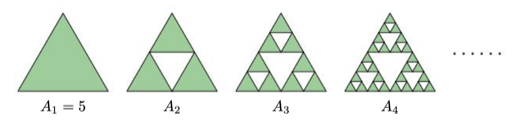
\includegraphics[scale=0.5]{images/sierpinski.png}
			\end{figure}
			\begin{enumerate}[label=\alph*)]
				\item Berechne $A_2$ und $A_3$.
				\item Bestimme eine explizite Formel für $A_n$.
				\item Ab welchem $n\in\N$ ist $A_n$ kleiner als $0.0001$?
				\item Wie viele eingefärbte Dreiecke hat das $n-$te Glied bei der Konstruktion solcher Dreiecke.
			\end{enumerate}
		\end{enumerate}
	\end{aufgabe}\newpage

\section{Unendliche geometrische Folgen und Reihen}
	Üblicherweise können Folgen unendliche viele Glieder haben. In diesem Abschnitt wollen wir vor allem die geometrischen Folgen in dieser Hinsicht untersuchen. Zuerst möchte ich aber anhand eines Beispiels zeigen, wieso diese Untersuchung für eine arithmetische Folge nicht interessant ist.
	\begin{beispiel}\ \\
		\begin{minipage}{0.5\linewidth}
			Betrachten wir also die arithmetische Folge \[a_n=-1+(n-1)\*\frac{1}{2}.\]
			\vspace{2.5cm}
		\end{minipage}
		\hfill
		\begin{minipage}{0.45\linewidth}
			\centering
			\begin{tikzpicture}[cross/.style={draw, cross out, minimum size=2*(#1-1pt), inner sep=0pt, outer sep=0pt}, x=1cm, y=1cm,
				>=latex,   %Voreinstellung für Pfeilspitzen
				font= \footnotesize, scale=0.6]
				%Raster zeichnen
				\draw [color=gray!50]  [step=10mm] (-0.3,-1.3) grid (10.3,5.3);
				% Achsen zeichnen
				\draw[->,thick] (-0.3,0) -- (10.8,0) node[right, below] {\normalsize $n$};
				\draw[->,thick] (0,-1.3) -- (0,5.8) node[above, left] {\normalsize $a_n$};
				% Achsen beschriften
				\foreach \x in {1,2,3,...,10} \draw (\x,-.1) -- (\x,.1) node[below=4pt] {$\x$};
				\foreach \y in {-1,1,2,3,...,5} \draw (-.1,\y) -- (.1,\y) node[left=4pt] {$\y$};
				% Besserer Ursprung
				\draw[color=black] (0pt,-14pt) node[right] {$0$};
				%Funktionen zeichnen:
				%\clip(-3.3,-5.3) rectangle (3.3,7.3); %Bildbereich
				%\draw[blue, smooth, domain=-9:9] plot (\x, {-1*pow(\x-3,2)+1}) node[yshift=13cm] {$$};
				%\draw[green, smooth, domain=-9:9] plot (\x, {2*pow(\x-3,2)-3}) node[] {$$};
				%\draw[red, smooth, domain=-9:9] plot (\x, {-0.4*pow(\x+3,2)+1}) node[right] {$$};
				%Beschriftung
				%\node[blue]  at (1,-5) {$p_2$};
			\end{tikzpicture}
		\end{minipage}
	\end{beispiel}
	\begin{aufgabe}
		Betrachte die geometrische Folge $1,2,4,8,16,\ldots$. Was können wir über ihre Partialsummen aussagen?
		\begin{table}[H]
			\centering
			\begin{tabular}{c|p{8mm}|p{8mm}|p{8mm}|p{8mm}|p{8mm}|p{12mm}|p{12mm}}
				$n$ & $1$ & $2$ & $5$ & $10$ & $20$ & $100$ & $1000$ \\\hline
				$s_n$ & & & & & & &
			\end{tabular}
		\end{table}
		Als Vergleich dazu betrachten wir die geometrische Folge $81,27,9,3,1,\ldots$.
		\begin{table}[H]
			\centering
			\begin{tabular}{c|p{8mm}|p{8mm}|p{8mm}|p{8mm}|p{8mm}|p{12mm}|p{12mm}}
				$n$ & $1$ & $2$ & $5$ & $10$ & $20$ & $100$ & $1000$ \\\hline
				$s_n$ & & & & & & &
			\end{tabular}
		\end{table}
		Was ist der Unterschied der beiden Folgen?\vspace{5pt}\newline\karos{5}
	\end{aufgabe}
	\begin{definition}
		Eine geometrische Reihe $\left(s_n\right)_{n\in\N}$ \textbf{konvergiert}, genau dann wenn ihre zugrunde liegende geometrische Folge $\left(a_n\right)_{n\in\N}$ gegen $0$ strebt.
		\[s_n\to s \Leftrightarrow a_n\to0 \quad\text{ für } n\to\infty\]
		Dabei wird $s$ als \textbf{Grenzwert der Reihe} bezeichnet.\newline
		Falls $a_n$ nicht gegen $0$ strebt, \textbf{divergiert} die Reihe.
	\end{definition}
	Da stellt sich uns natürlich jetzt die Frage, kann dieser Grenzwert der Reihe berechnet werden? Um dies untersuchen, müssen wir also verstehen, welchen Einfluss sehr grosse $n$ in der Formel \[s_n=a_1\*\frac{q^n-1}{q-1}\] haben.
	Dazu unterscheiden wir drei Fälle:
	\begin{enumerate}[label=\arabic*. Fall:]
		\item $\mathbf{\abs{q}>1}$\newline
		Beispiel: $1+2+4+8+16\ldots \quad\Rightarrow\quad q=\gap{2}$\newline
		\[s_n=a_1\*\frac{q^n-1}{q-1}\]
		\item $\mathbf{\abs{q}=1}$\newline
		Beispiel: $1+1+1+1+1+\ldots \quad\Rightarrow\quad q=\gap{2}$\newline
		Beispiel: $1-1+1-1+1-\ldots \quad\Rightarrow\quad q=\gap{2}$\newline
		\[s_n=a_1\*\frac{q^n-1}{q-1}\]
		\item $\mathbf{\abs{q}<1}$\newline
		Beispiel: $81+27+9+3+1+\ldots \quad\Rightarrow\quad q=\gap{2}$\newline
		\[s_n=a_1\*\frac{q^n-1}{q-1}\]
	\end{enumerate}
	\begin{satz}[Grenzwert einer unendlichen geometrischen Reihe]
		Der Grenzwert einer unendlichen geometrischen Reihe kann wie folgt berechnet werden:
		\begin{enumerate}[label=\ ]
			\item $\abs{q}>1$:
			\item $\abs{q}=1$:
			\item $\abs{q}<1$: s=
		\end{enumerate}
	\end{satz}
	Der Begriff des Grenzwertes wird im folgenden Kapitel noch ausführlicher thematisiert und untersucht.
	\begin{aufgabe}
		\begin{enumerate}
			\item Berechne den Grenzwert der unendlichen geometrischen Reihen, falls er existiert. %DMK Ana S11 A62a_f
			\begin{enumcols}[3]
				\item $\displaystyle 6+2+\frac{2}{3}+\ldots$
				\item $\displaystyle 1-\frac{5}{4}+\frac{25}{16}-\frac{125}{64}+\ldots$
				\item $\displaystyle\sum_{i=0}^\infty\left(\frac{-7}{8}\right)^k$
			\end{enumcols}
			\item Betrachte die Partialsumme $\displaystyle s_n=1+\frac{9}{10}+\left(\frac{9}{10}\right)^2+\ldots+\left(\frac{9}{10}\right)^{n-1}$. %DMK Ana S11 A63
			\begin{enumerate}[label=\alph*)]
				\item Wie lautet die explizite Formel für die Partialsumme $s_n$?
				\item Wie gross ist die Summe der ersten $100$ Gliedern?
				\item Berechne den Grenzwert der unendlichen geometrischen Reihe.
			\end{enumerate}
			\item Von einer geometrischen Reihe sind $a_5=0.0972$ und $q=0.3$ bekannt. Berechne den Grenzwert $s$. %DMK Ana S11 A64
			\item Bestimme den Quotienten $q$ einer unendlichen geometrischen Reihe, wenn der Grenzwert $s$ $6-$mal so gross wie das erste Glied ist. %DMK Ana S11 A66a
			\item Einem Quadrat mit Seitenlänge $s=1$ werden weitere Quadrate einbeschrieben, indem man die jeweiligen Seitenmittelpunkte eines Quadrates miteinander verbindet. Berechne den Gesamtinhalt aller Quadratflächen.
			\item Einem Quadrat mit Seitenlänge $s=1$ wächst wie im Bild unten neue Quadrate, deren Seitenlänge jeweils $\displaystyle\frac{1}{3}$ der alten sind.
			\begin{figure}[H]
				\centering
				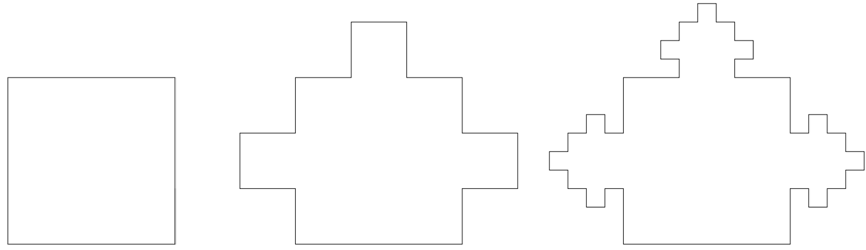
\includegraphics[scale=0.5]{images/quadratpflanze.png}
			\end{figure}
			\begin{enumerate}[label=\alph*)]
				\item Wird die Fläche unendlich gross? Begründe.
				\item Wird der Umfang unendlich lang? Begründe.
			\end{enumerate}
			\item Ein spiralförmiger Weg beginnt beim Ursprung $(0,0)$ und besteht aus Strecken (wie abgebildet), die eine geometrische Folge bilden.\newline %DMK Ana S12 A73
			\begin{minipage}{0.6\linewidth}
				\begin{enumerate}[label=\alph*)]
					\item Wie lang ist der unendlich fortgesetzte Weg?
					\item Wo liegt der Zielpunkt $Z$ dieses Weges?
				\end{enumerate}
			\end{minipage}
			\hfill
			\begin{minipage}{0.35\linewidth}
				\centering
				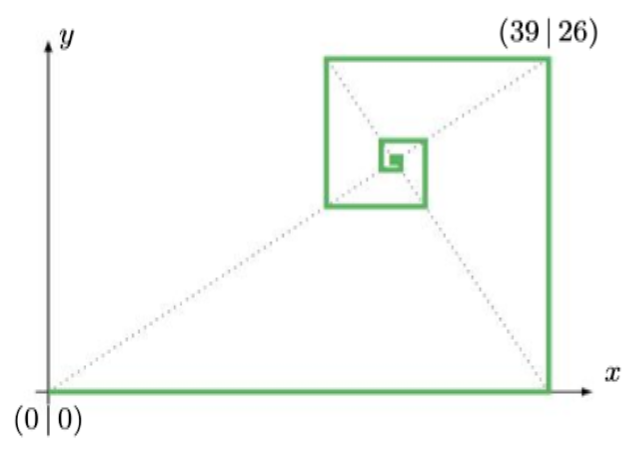
\includegraphics[scale=0.2]{images/spiralweg.png}
			\end{minipage}
		\end{enumerate}
	\end{aufgabe}


\newpage
\subsection*{History}
\begin{table}[H]
	\centering
	\begin{tabular}{|p{13mm}|p{20mm}|p{30mm}|p{70mm}|}\hline
		%\multicolumn{4}{|l|}{History}\\\hline
		Version & Datum & Person & Bemerkung \\\hline
		$0.1$ & 02.08.2024 & Jonas Guler & Kapitel erstellt \\\hline
		$1.0$ & 01.04.2025 & Jonas Guler & Kapitel fertig \\\hline
	\end{tabular}
\end{table}


\end{document}